Para evaluar el desempeño empírico de las implementaciones, se llevó a cabo una serie de pruebas en las que se midieron dos métricas fundamentales de rendimiento:
\begin{enumerate}
    \item \textbf{Tiempo de Ejecución (ms):} Registrado mediante la librería \texttt{std::chrono::high\_resolution\_clock}, 
    aislando exclusivamente el tiempo de cómputo algorítmico respecto al tamaño de la entrada $N$.
    \item \textbf{Uso de Memoria Máxima Residente (KB):} Cuantificado a través de la llamada al sistema \texttt{wait4()} y la estructura \texttt{rusage} (\textit{ru\_maxrss}), asegurando registrar el pico de memoria física del proceso hijo independiente para cada ejecución.
\end{enumerate}

La automatización de la toma de muestras y la generación de visualizaciones (gráficos y tablas) se realizó mediante scripts en Python (\texttt{plot\_generator.py}) integrados en los flujos de compilación (\texttt{Make}), garantizando la trazabilidad y fidelidad entre los datos generados por las implementaciones en C++ y las gráficas presentadas.

\subsection{Algoritmos de Ordenamiento}

Se evaluaron cuatro algoritmos de ordenamiento con distintas naturalezas teóricas: \textbf{MergeSort} (basado en \textit{Dividir y Conquistar}), \textbf{QuickSort} (partición \textit{in-place}), \textbf{PatienceSort} (basado en la formación de pilas y colas de prioridad), y el algoritmo altamente optimizado de la biblioteca estándar de C++ (\textsc{std::sort}). Las pruebas consideraron arreglos de tamaños desde $N = 10$ hasta $N = 10^7$ elementos bajo distribuciones ascendentes, descendentes y aleatorias.

\subsubsection{Tiempos de Ejecución y Complejidad Temporal}

En la Figura 1 y en el Cuadro 1 se observa el crecimeinto exponencial logaritmico característico de la familia de ordenamiento óptimo por comparación $\Theta(N log N)$.

\noindent
\begin{figure}[H]
    \centering
    % Columna izquierda: Gráfico más grande (57% del ancho)
    \begin{minipage}[c]{0.57\textwidth}
        \centering
        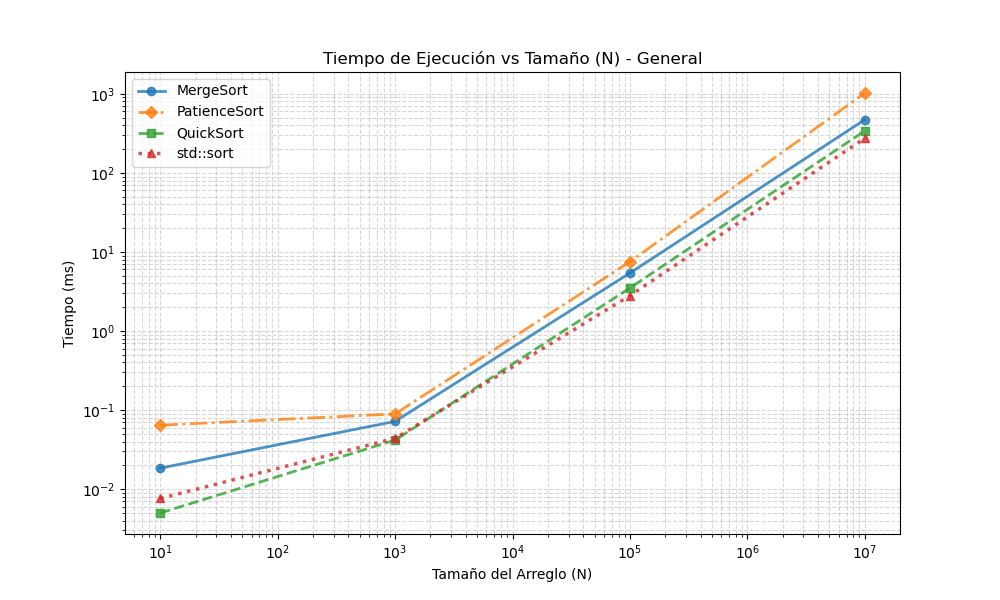
\includegraphics[width=\linewidth]{sections/Array_tiempo_ejecucion_general.png}
        \caption{Tiempo de ejecución vs. $N$ para los cuatro algoritmos de ordenamiento.}
        \label{fig:sort_tiempo_general}
    \end{minipage}\hfill
    % Columna derecha: Tabla ajustada (40% del ancho)
    \begin{minipage}[c]{0.40\textwidth}
        \centering
        \footnotesize
        \setlength{\tabcolsep}{3pt} % Reduce el padding entre columnas para que entre mejor
        \resizebox{\linewidth}{!}{%
            \begin{tabular}{|l|l|r|r|r|}
                \hline
                \textbf{Algoritmo} & \textbf{Tipo} & \textbf{Tamaño ($N$)} & \textbf{Tiempo (ms)} & \textbf{Memoria (KB)} \\ \hline
                MergeSort    & Aleatorio & $10^5$ & 5.03   & 2864  \\ \hline
                QuickSort    & Aleatorio & $10^5$ & 2.87   & 2792  \\ \hline
                PatienceSort & Aleatorio & $10^5$ & 3.18   & 3196  \\ \hline
                std::sort    & Aleatorio & $10^5$ & 2.76   & 2820  \\ \hline
                MergeSort    & Aleatorio & $10^7$ & 528.26 & 81032 \\ \hline
                QuickSort    & Aleatorio & $10^7$ & 286.92 & 42856 \\ \hline
                PatienceSort & Aleatorio & $10^7$ & 483.75 & 120332 \\ \hline
                std::sort    & Aleatorio & $10^7$ & 214.41 & 41448 \\ \hline
            \end{tabular}%
        }
        \captionof{table}{Rendimiento de ordenamiento con entradas aleatorias.}
        \label{tab:ordenamiento_simple}
    \end{minipage}
\end{figure}

\texttt{std::sort} y \texttt{QuickSort} demuestran el mejor rendimiento constante en la practica. El primero sobresale gracias a sus optimizaciones a nivel de compilador y el uso hibrido de algoritmos, cambiando a \textit{Insertion Sort} para subarrays pequeños y \textit{Heapsort} para evitar peores casos cuadráticos. Por otro lado, \textit{Quicksort} muestra un excelente desempeño promedio, aunque es sensible a la elección del pivote en instancias altamente estructuradas.\\

\texttt{MergeSort} muestra un comportamiento sumamente predecible y estable $\Theta(N log N)$ en todas las configuraciones de entrada (ascendente, descendente y aleatorio), lo que es fiel al balance teórico de su árbol de recursión y su recurrencia asociada ($T(N) = 2T(N/2) + \Theta(N)$). Sin embargo, experimenta una constante multiplicativa mayor debido a la constante transferencia de datos hacia arreglos auxiliares.\\

Por último, \texttt{PatienceSort} si bien parcticamente opera en $\Theta(N log N)$, debido a que requiere $N$ inserciones en colas de prioridad basadas en \textit{heaps} de tamaño asintótico menor o igual al número de pilas, en la práctica presenta un tiempo de ejecución superior en entradas masivas ($N = 10^7$), tal como se puede obsrvar en la figura 1, debido a la sobrecarga por la gestión dinámica de múltiples estructuras de datos auxiliares (vectores de punteros y colas de prioridad \texttt{std::priority\_queue}.

\subsubsection{Análisis de Consumo de Memoria}

El comportamiento espacial, ilustrado en la figura 2 y resumido en el Cuadro 1, refleja fielmente las diferencias teóricas de espacio auxiliar entre los algoritmos:

\begin{figure}[H]
    \centering
    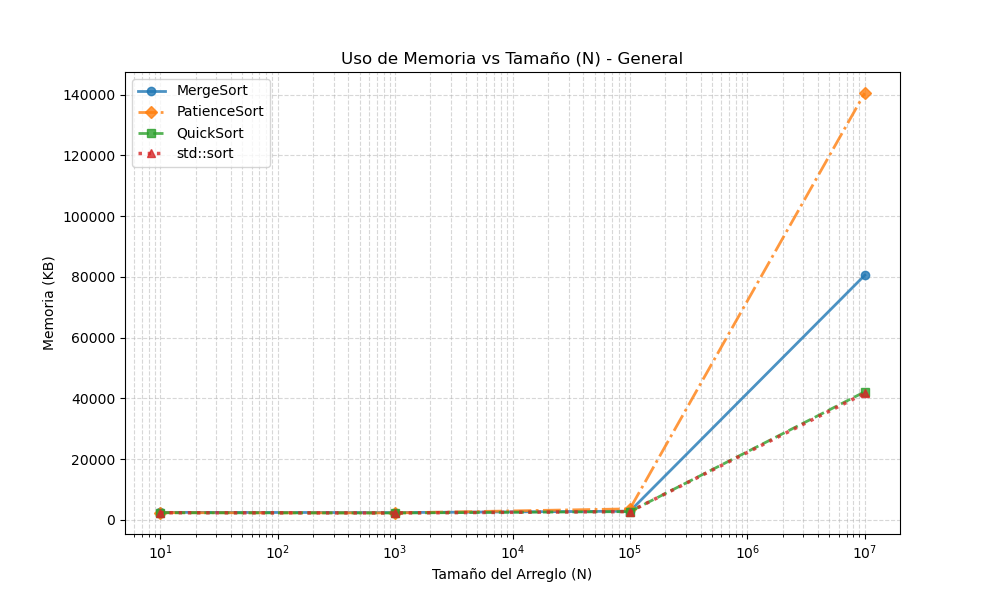
\includegraphics[width=0.50\textwidth]{sections/Array_uso_memoria_general.png}
    \caption{Tiempo de ejecución vs. $N$ para los cuatro algoritmos de ordenamiento.}
    \label{fig:sort_tiempo_general}
\end{figure}

\texttt{QuickSort} y \texttt{std::sort} operan como algoritmos de memoria auxiliar mínima, requiriendo únicamente espacio proporcional a la profundidad del árbol de recursion ($\Theta(log N)$ en promedio). Para $N = 10^7$, la huella de memoria se mantiene estable en torno a los $41-43 MB$, lo que coincide casi con exactitud con el tamaño base del vector en RAM.\\

\texttt{MergeSort} exhibe una cota de espacio auxiliar de $\Theta(N)$ al necesitar un arreglo temporal contiguo de igual magnitud para intercalar las mitades, uplicando el consumo de memoria respecto al vector original (alcanzando $81.032 KB$ en $N = 10^7$).\\

\texttt{PatienceSort} Registra el consumo espacial más elevado de todas las alternativas de ordenamiento ($120.332 KB$ en $N = 10^7$). Esto se explica por la estructura enlazada de nodos (\textit{next\_node}), los vectores auxiliares de cabeceras de pila y la sobrecarga interna del contenedor de prioridad

\subsection{Algoritmos de Multiplicación de Matrices}

Se contrastó el algoritmo iterativo clásico (\textbf{Naive}) frente al método recursivo de \textbf{Strassen} obre matrices cuadradas con dimensiones $N \in \{16, 64, 256, 1024\}$ bajo estructuras densas, diagonales y dispersas

\subsubsection{Tiempos de Ejecución y Complejidad Temporal}

En la Figura 3  y en el Cuadro 2 se exponen los resultados promedio obtenidos para matrices densas.

\noindent
\begin{figure}[H]
    \centering
    % Columna izquierda: Gráfico
    \begin{minipage}[c]{0.56\textwidth}
        \centering
        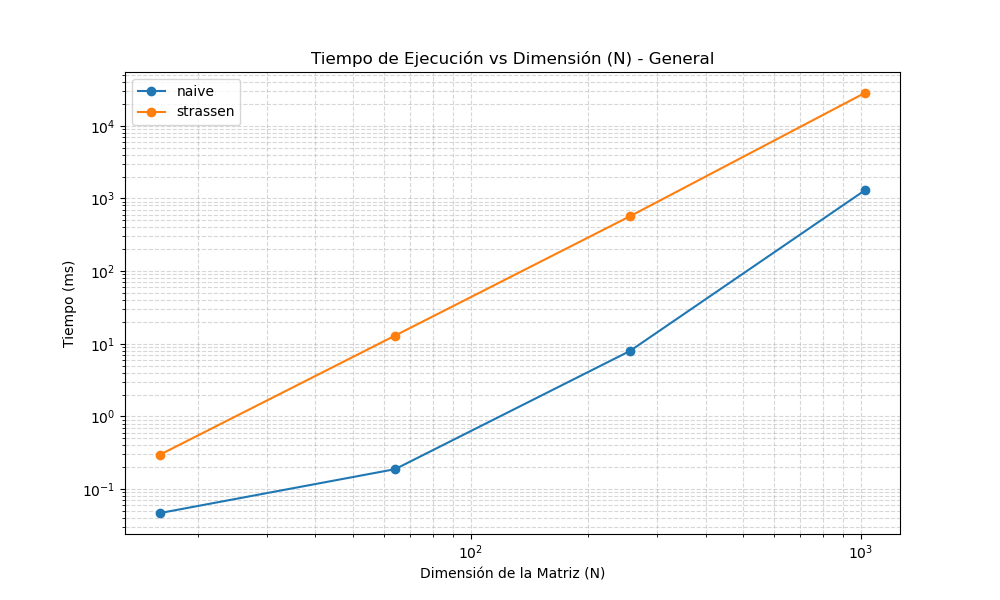
\includegraphics[width=\linewidth]{sections/Matrix_tiempo_ejecucion_general.png}
        \caption{Tiempo de ejecución vs. Dimensión $N$ para multiplicación de matrices (Promedio General).}
        \label{fig:matrix_tiempo_general}
    \end{minipage}\hfill
    % Columna derecha: Tabla
    \begin{minipage}[c]{0.41\textwidth}
        \centering
        \footnotesize
        \setlength{\tabcolsep}{3pt}
        \resizebox{\linewidth}{!}{%
            \begin{tabular}{|l|rr|rr|}
                \hline
                \textbf{Dimensión ($N$)} & \multicolumn{2}{c|}{\textbf{Tiempo (ms)}} & \multicolumn{2}{c|}{\textbf{Memoria (KB)}} \\ \cline{2-5}
                & \textbf{Naive} & \textbf{Strassen} & \textbf{Naive} & \textbf{Strassen} \\ \hline
                $16 \times 16$     & 0.03    & 0.29      & 2\,592  & 2\,592  \\ \hline
                $64 \times 64$     & 0.18    & 11.60     & 3\,040  & 3\,004  \\ \hline
                $256 \times 256$   & 7.79    & 574.67    & 3\,440  & 4\,512  \\ \hline
                $1024 \times 1024$ & 1\,311.43 & 28\,807.50 & 15\,072 & 46\,064 \\ \hline
            \end{tabular}%
        }
        \captionof{table}{Comparativa de rendimiento en matrices densas ($N \times N$).}
        \label{tab:matrices}
    \end{minipage}
\end{figure}

Los datos empíricos permiten identificar dos fenómenos teóricos fundamentales:
\begin{itemize}
    \item \textbf{Dominancia de Naive en dimensiones prácticas ($N \le 1024$):} El análisis asintótico formal determina que Strassen reduce la recurrencia a $T(N) = 7T(N/2) + \Theta(N^2)$, lo que por Teorema Maestro produce una complejidad subcúbica de $\Theta(N^{\log_2 7}) \approx \Theta(N^{2.8073})$,  teóricamente superior a la cota cúbica $\Theta(N^3)$ de Naive. Sin embargo, en la práctica el algoritmo Naive supera con holgura a Strassen en todas las dimensiones evaluadas (por ejemplo, para $N = 256$, Naive toma ~7.79 ms contra los ~574.67 ms de Strassen)

    \item \textbf{Sobrecarga de combinación y asignación recursiva:} Strassen ahorra una multiplicación escalar por nivel a costa de ejecutar 18 sumas y restas de matrices de tamaño $(N/2) \times (N/2)$. En una arquitectura word-RAM real, la subdivisión y combinación de submatrices exige constantes reservas, liberaciones y copias en memoria dinámica. Estas operaciones introducen una constante multiplicativa oculta sumamente pesada que neutraliza la ventaja asintótica en dimensiones intermedias, justificando la necesidad de aplicar umbrales híbridos que deriven el cómputo a Naive cuando $N$ desciende por debajo de un valor límite.
\end{itemize}

\subsubsection{Análisis de Consumo de Memoria}

\begin{figure}[H]
    \centering
    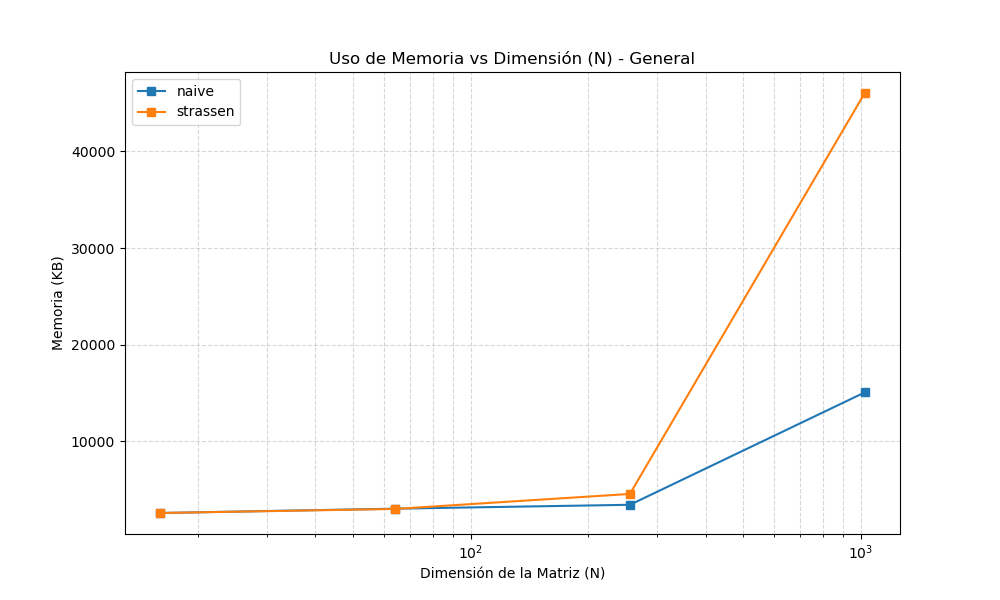
\includegraphics[width=0.50\textwidth]{sections/Matrix_uso_memoria_general.png}
    \caption{uso de memoria vs. $N$ para las matrices.}
    \label{fig:sort_tiempo_general}
\end{figure}

De acuerdo con las mediciones ilustradas en la figura 4 sobre el uso de memoria de los algoritmos se tiene que:
\begin{itemize}
    \item \textbf{Naive:} Presenta una utilización espacial óptima $\Theta(N^2)$ circunscrita a la matriz resultante. En $N = 1024$ consume únicamente 15.072 KB de memoria física, manteniendo un espacio de trabajo estático libre de sobrecarga en la pila de llamadas
    \item \textbf{Strassen:} Triplica el uso de memoria residente alcanzando 46.064 KB para $N = 1024$. Este incremento sistemático proviene de la coexistencia de las submatrices temporales ($A, B, \dots, H$, $P_1, \dots, P_7$) creadas simultáneamente a lo largo de los distintos niveles de profundidad del árbol de recursión antes de combinarse en los cuadrantes finales
\end{itemize}
